\documentclass[11pt]{article}
\usepackage[preprint]{acl}

\usepackage{times}
\usepackage{latexsym}
\usepackage[T1]{fontenc}
\usepackage[utf8]{inputenc}
\usepackage{microtype}
\usepackage{inconsolata}
\usepackage{graphicx}
\usepackage{booktabs}

\title{Confidence Before Competence: Entity Frequency and Calibration\\ During Language Model Pretraining}

\author{Tomer Zalberg \\ Tel Aviv University \\ \texttt{tomerzalberg@mail.tau.ac.il} \\\And
  Chen Mizrahi \\ Tel Aviv University \\ \texttt{chenmizrahi2@mail.tau.ac.il} \\\AND
  Ofek Tovli \\ Tel Aviv University \\ \texttt{ofektovli@mail.tau.ac.il} \\\And
  Victoria Shabanov \\ Tel Aviv University \\ \texttt{shabanov@mail.tau.ac.il} \\}

\begin{document}
\maketitle

\begin{abstract}
A language model that gets a fact wrong is only dangerous if it sounds sure. We ask how the
number of times a fact appeared in pretraining affects the match between a model's confidence
and its accuracy, and when during pretraining that relationship forms. We use LMEnt
\citep{gottesman-etal-2026-lment}, which releases language models together with the
entity-annotated corpus they were trained on, so the number of times a subject and its answer
co-occurred is known rather than estimated. Scoring 2{,}993 PopQA facts on 61 checkpoints across
four models, we find that a randomly initialised model already
reports a confidence-accuracy gap of about $0.13$, and that training closes it in proportion to
exposure: by $0.28$ for facts with 61 to 200 co-occurrences, while leaving it unchanged for
facts whose entities never co-occur. The ordering holds under all three scoring functions we tried, though
the levels do not. The gap is already present at step 1{,}000 of 658{,}032, where confidence
varies far less across frequency than accuracy does: across the ten bins accuracy rises by
$0.275$ and confidence by $0.076$. Neither model scale from 170M to 1B, nor six epochs instead of one, nor
rephrased prompts remove the effect. When the model is wrong it tends to fall back on the most
likely answer for the relation, and it does so more often for rare entities. Our code, probe set
and per-checkpoint results are released.
\end{abstract}

\section{Introduction}

Language models store a lot of facts, and they store them unevenly. Facts about widely discussed
entities are recalled well; facts about rare ones are not
\citep{mallen-etal-2023-trust, kandpal-etal-2023-large}. Less is known about what the model does
when recall fails. It could spread probability evenly over the options, which would tell a user
that it does not know, or it could commit to one wrong answer, which would not.

This paper measures which of those happens, as a function of how often the fact appeared in
pretraining and how far training has progressed. Both questions need something that
is normally unavailable: the training corpus of the model under test, annotated well enough to
count how often two entities appeared together. LMEnt \citep{gottesman-etal-2026-lment} provides
exactly that, along with intermediate checkpoints, so we can count occurrences instead of
approximating them with a popularity proxy.

We score 2{,}993 PopQA facts as ten-way multiple choice at each checkpoint and record two numbers
per fact: whether the model picks the gold answer, and how much probability it puts on its
choice. Averaged over facts with the same co-occurrence count, the difference between the two is
a simple measure of how far confidence runs ahead of knowledge.

Three findings follow. First, that difference tracks co-occurrence count closely, and it is not
present in a randomly initialised model, so training produces it. Second, it appears very early:
by step 1{,}000 of 658{,}032 the model is about equally confident about facts it has never seen
evidence for and facts it has seen hundreds of times, even though its accuracy on the two groups
already differs by a factor of two and a half. Confidence arrives before the knowledge it is supposed to reflect. Third, the effect survives every control we ran, including a six-fold
increase in model size.

\begin{figure*}[t]
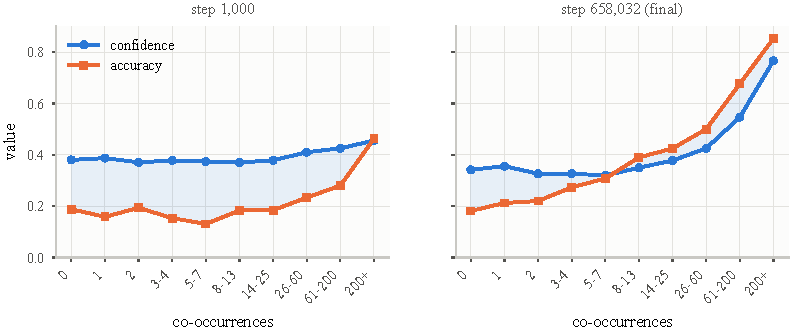
\includegraphics[width=\textwidth]{figures/fig8_early_uniform_confidence.pdf}
\caption{Confidence and accuracy by co-occurrence count, early in training and at the end.
At step 1{,}000 confidence is nearly flat across frequency while accuracy is not. The shaded
region is the gap between them.}
\label{fig:main}
\end{figure*}

\section{Background}

\paragraph{Frequency and factual recall.}
\citet{kandpal-etal-2023-large} entity-link five pretraining corpora and count documents
containing both the question and answer entities, then show strong correlational and causal relationships
between that count and question-answering accuracy. They also estimate that models would need to
be scaled by many orders of magnitude before they answer well on questions with little support in
pretraining. \citet{mallen-etal-2023-trust} introduce PopQA, 14k questions about long-tail
entities, and report that scaling mainly improves recall of popular knowledge and does little for
the tail. Both papers measure accuracy. Neither asks what the model's confidence does.

\paragraph{Knowledge during pretraining.}
\citet{chang-etal-2024-large} study acquisition directly by injecting facts a model has not seen
into intermediate checkpoints and tracking how the probability of those facts rises and then
decays. They report a power-law relation between training steps and forgetting, faster forgetting
when training data is duplicated, and greater robustness at larger batch sizes. Because they
inject facts, their design controls exposure precisely but does not measure facts the model met
naturally. We take the complementary route and observe naturally occurring facts whose corpus
counts are known.

\paragraph{LMEnt.}
LMEnt \citep{gottesman-etal-2026-lment} releases a Wikipedia-based pretraining corpus annotated
with entity mentions, an entity-based retrieval method over that corpus, and pretrained models of
up to 1B parameters with intermediate checkpoints. Among several candidate predictors of model
accuracy they find that Subject-Answer Chunks, defined as the number of corpus chunks in which
the subject and answer entities co-occur, correlates most strongly with performance, better than
Wikipedia pageview popularity. They also analyse knowledge acquisition over training, evaluating
their 1B model every 20K steps and marking a fact as learned when the model answers at least one
question linking the subject to the answer. They report that rates of both learning and
forgetting rise with fact frequency, and close by noting that the interplay between internal
mechanisms and training dynamics is not yet fully understood. Their analysis is framed in terms
of whether a fact is known. We use the same resource to ask a different question about the same
checkpoints, namely how sure the model is.

\paragraph{Calibration.}
A calibrated classifier assigns confidence equal to its probability of being correct.
\citet{guo-etal-2017-calibration} show that modern neural networks are poorly calibrated and
summarise miscalibration with expected calibration error
\citep{naeini-etal-2015-obtaining}. That statistic is unsigned. We report the signed difference
between mean confidence and mean accuracy instead, because the direction is what we are after: a
model that is too sure and one that is not sure enough are different failures. Scoring multiple-choice options by raw string probability is also known to be
unreliable, because surface forms compete for probability mass
\citep{holtzman-etal-2021-surface}. Section~\ref{sec:scoring} shows this matters here.
Closer to our setting, \citet{desai-durrett-2020-calibration} find that fine-tuned BERT and
RoBERTa classifiers are calibrated in-domain and degrade out-of-domain, while staying better
calibrated than models trained from scratch, and \citet{kadavath-etal-2022-language} report that
large models are well calibrated on multiple-choice questions when the options are presented in a
suitable format, and can partly predict whether they know an answer at all. Both study
fully trained models. We ask when that calibration arrives during pretraining, and whether it
holds for facts the corpus barely contains.

\section{Experimental Setup}

\subsection{Facts and frequency}

We use the PopQA subset released with LMEnt, which pairs each question with the identifiers of
the chunks where the subject entity, the answer entity, and both together appear. The
co-occurrence count is the paper's Subject-Answer Chunks measure. We sort the 14{,}267 facts by
that count and split them into ten value-based bins, which therefore differ in size, then
sample 300 facts per bin, giving 2{,}993 facts
after discarding a handful for which we could not build a full candidate set. Bin edges and
counts are in Table~\ref{tab:data}.

Two groups deserve mention. In the lowest bin the subject and answer never co-occur, so the
corpus contains no direct evidence for the fact. For 112 of those facts the subject entity is
absent from the corpus altogether, a stricter control we report separately.

\begin{table}[t]
\centering\small
\begin{tabular}{lrrr}
\toprule
\textbf{Co-occurrences} & \textbf{Available} & \textbf{Sampled} & \textbf{Test} \\
\midrule
0 & 2450 & 298 & 85 \\
1 & 2307 & 297 & 83 \\
2 & 1586 & 300 & 75 \\
3--4 & 1999 & 300 & 61 \\
5--7 & 1556 & 299 & 83 \\
8--13 & 1437 & 300 & 70 \\
14--25 & 985 & 299 & 70 \\
26--60 & 769 & 300 & 90 \\
61--200 & 522 & 300 & 65 \\
200+ & 656 & 300 & 75 \\
\midrule
Total & 14267 & 2993 & 757 \\
\bottomrule
\end{tabular}
\caption{Facts per co-occurrence bin. Splits are 50/25/25 over 2{,}826 distinct subject entities,
so no entity appears in more than one split. Only the prediction task in Section~\ref{sec:pred}
uses the splits. Everything else is measured over all 2{,}993 facts.}
\label{tab:data}
\end{table}

\subsection{Probes}

Each of the 16 PopQA relations gets one hand-written cloze template, for example
\textit{The director of \{subject\} is}. Templates are fixed in advance and applied
mechanically, so probe construction is reproducible and involves no model in the loop.

For each fact we build a ten-option multiple choice question: the gold answer plus nine
distractors drawn from the objects observed for the same relation, so all options are
type-consistent. Distractors are matched to the gold on token length, which limits the
length bias described below, and screened against the gold's alias list so no distractor
is silently correct. Mean gold length is 2.95 tokens against 2.93 for distractors. Chance
accuracy is 0.100.

\subsection{Scoring}
\label{sec:scoring}

We score each option by its length-normalised log probability under the prompt and take a softmax
over the ten options. Accuracy is whether the gold option ranks first; confidence is the
probability of the top-ranked option.

The choice of scoring function decides what confidence even means here. At step 0 the model's weights are
random, so whatever confidence a scorer reports there is floor rather than belief. The three
disagree sharply: summed log probability reports 0.439, because it ranks options largely by how
short they are, domain-conditional PMI \citep{holtzman-etal-2021-surface} reports 0.396, and
length-normalised scoring reports 0.216. We use length-normalised scoring throughout, because the
lowest floor leaves the most room to detect confidence that reflects knowledge, and we report the
other two alongside it.

We also record a free-generation probe: greedy decoding of ten tokens from the same prompt,
scored by normalised string match against the answer aliases, with the mean token log probability
of the generated span as its confidence.

\subsection{Models}

We evaluate the LMEnt models at 170M, 600M and 1B parameters trained for six epochs, and the 1B
model trained for one epoch. Of the checkpoints LMEnt describes, we use those publicly released
on HuggingFace: 25 for the 1B six-epoch model, including every 1{,}000 steps over the first
10{,}000, and 12 each for the others. That gives 61 checkpoint evaluations, plus six more for the
template controls, two alternative wordings at three checkpoints of the 1B model. All inference runs in float32, because the 1B model's activations reach
roughly $3\times10^{6}$, far above the float16 range, and float16 produces non-finite scores on
every trained checkpoint. Total compute is about 8 GPU-hours on Tesla T4s.

The probe set is fixed by a seed and identified by the hash \texttt{5132e8b6ffaa40cb}. Every run
verifies it before scoring. We release the notebooks, the 2{,}993-fact probe set, and per-fact
results for all 67 runs, along with a manifest per run recording the GPU, numeric precision and
library versions used, at \url{https://github.com/TomerZ1/confidence-before-competence}.

\section{Results}

\subsection{Confidence outruns accuracy for rare facts}

Figure~\ref{fig:main} shows confidence and accuracy against co-occurrence count at step 1{,}000
and at the end of training. At step 1{,}000 the two curves are almost independent: accuracy
already rises by 0.275 across the bins while confidence rises by 0.076. Over the seven rarest
bins both are flat, at 0.130 to 0.193 and 0.370 to 0.387. The model is then close to equally
sure about facts it has no evidence for and facts it has seen a few dozen times, while being
wrong about most of both.

By the end of training the curves have partly converged, but a gap remains at the rare end.
Figure~\ref{fig:gap} plots the difference. It falls steadily from $+0.160$ in the lowest bin to
$-0.130$ in the second-highest, crossing zero between 5--7 and 8--13 co-occurrences. Beyond that
point the model is underconfident: it is right more often than it claims. Where the crossing
falls, and whether it happens at all, depends on the scoring function. Under PMI no bin is
negative. The decline across frequency is the same under all three
(Table~\ref{tab:robust}). Rank correlation between log co-occurrence count and the per-fact
gap is $-0.253$ for length-normalised scoring, $-0.287$ for summed and $-0.206$ for PMI, with
$p < 10^{-29}$ in every case.

The same measurement on the randomly initialised checkpoint is flat, between 0.100 and 0.156,
with no ordering by frequency. That floor is not zero, because the largest of ten softmax
probabilities exceeds 0.100 by construction. Measured against it, training closes the gap by
0.284 for facts with 61 to 200 co-occurrences, while leaving it statistically unchanged for facts
whose entities never co-occur: the gap there moves by $+0.009$, and the initial value of 0.151
sits inside the final bootstrap interval of [0.117, 0.202]. The change is almost perfectly
ordered by frequency (Spearman $-0.98$). The model does not learn to be overconfident about rare
facts. It begins overconfident about everything, and exposure is what corrects it, except where
there is nothing to correct it with.


\begin{figure}[t]
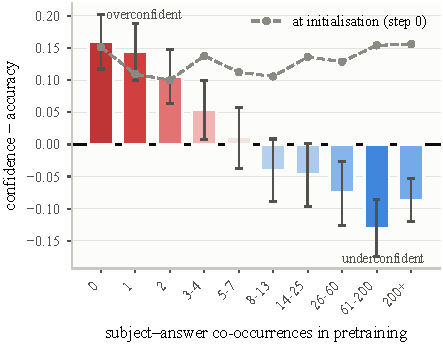
\includegraphics[width=\columnwidth]{figures/fig1_gap_by_exposure.pdf}
\caption{Confidence minus accuracy at the final checkpoint of the 1B six-epoch model. Error bars
are bootstrap 95\% intervals over facts. The dashed line is the same quantity at initialisation
and is the reference the trained values should be read against, not zero.}
\label{fig:gap}
\end{figure}

\begin{table}[t]
\centering\small
\setlength{\tabcolsep}{4.5pt}
\begin{tabular}{lrrrrr}
\toprule
& \multicolumn{4}{c}{\textbf{Gap by co-occurrence}} & \\
\cmidrule(lr){2-5}
\textbf{Scoring} & 0 & 5--7 & 26--60 & 200+ & $\rho$ \\
\midrule
Length-norm. & 0.160 & 0.012 & -0.075 & -0.087 & -0.25 \\
Summed       & 0.385 & 0.310 &  0.175 & -0.009 & -0.29 \\
PMI          & 0.398 & 0.355 &  0.282 &  0.074 & -0.21 \\
\bottomrule
\end{tabular}
\caption{Confidence minus accuracy at the final checkpoint, at four representative bins, under
each scoring function. $\rho$ is the rank correlation between log co-occurrence count and the
per-fact gap over all 2{,}993 facts. The level shifts and the sign is not preserved, but the
decline across frequency is.}
\label{tab:robust}
\end{table}

\subsection{Confidence settles early, accuracy does not}

Pooled over all facts, confidence moves from 0.216 at initialisation to 0.393 at step 1{,}000 and
then spans 0.038 across the remaining 657{,}000 steps, a net change of 0.021, while accuracy rises by 0.187
over the same span. That pooled summary hides something, so we report the bins separately in
Table~\ref{tab:change}: confidence falls slightly for rare facts and rises steeply for frequent
ones, and the two movements cancel. Accuracy rises almost everywhere.

The dissociation is clearest in the middle bins. For facts with 8--13 co-occurrences, accuracy
improves by 0.207 after step 1{,}000 while confidence moves by $-0.020$. For the most frequent
facts, confidence and accuracy rise together and stay close. Trajectories are in
Figure~\ref{fig:traj}.

\begin{table}[t]
\centering\small
\begin{tabular}{lrrrr}
\toprule
& \multicolumn{2}{c}{\textbf{Confidence}} & \multicolumn{2}{c}{\textbf{Accuracy}} \\
\cmidrule(lr){2-3}\cmidrule(lr){4-5}
\textbf{Co-occ.} & 1K & final & 1K & final \\
\midrule
0      & 0.380 & 0.341 & 0.188 & 0.181 \\
1      & 0.387 & 0.356 & 0.158 & 0.212 \\
2      & 0.371 & 0.326 & 0.193 & 0.220 \\
3--4   & 0.378 & 0.327 & 0.153 & 0.273 \\
5--7   & 0.373 & 0.319 & 0.130 & 0.308 \\
8--13  & 0.370 & 0.350 & 0.183 & 0.390 \\
14--25 & 0.378 & 0.377 & 0.184 & 0.425 \\
26--60 & 0.410 & 0.425 & 0.233 & 0.500 \\
61--200& 0.425 & 0.546 & 0.280 & 0.677 \\
200+   & 0.456 & 0.767 & 0.463 & 0.853 \\
\bottomrule
\end{tabular}
\caption{Confidence changes little after step 1{,}000 except at the frequent end, where it
tracks a large accuracy gain. Accuracy improves across almost all bins.}
\label{tab:change}
\end{table}

\begin{figure*}[t]
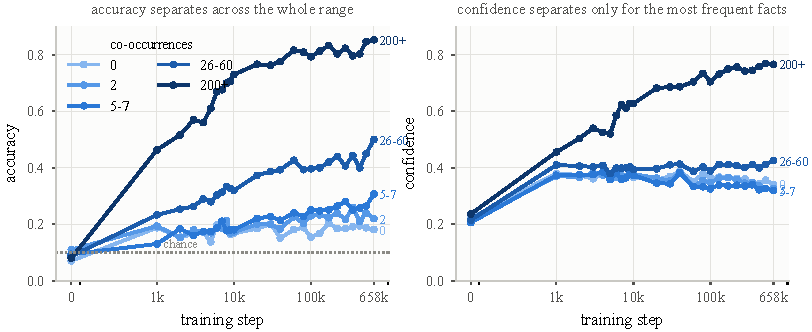
\includegraphics[width=\textwidth]{figures/fig3_dissociation.pdf}
\caption{Accuracy and confidence over training for five representative bins. Accuracy separates
across the whole frequency range; confidence separates only at the frequent end.}
\label{fig:traj}
\end{figure*}

\subsection{Controls}

Figure~\ref{fig:controls} repeats the final-checkpoint gap under three changes. Increasing model
size from 170M to 1B leaves the rare-end gap essentially where it was, at 0.197, 0.158 and 0.160
respectively. Training the 1B model for one epoch instead of six gives a curve close to the
six-epoch one, so repeated passes over the same corpus do not improve the match between
confidence and accuracy. Two rephrasings of every template, one passive and one possessive,
reproduce the same shape, so the effect is not an artefact of our wording.

We compare the one-epoch and six-epoch models at their final checkpoints rather than at equal
step counts, because the two use different learning-rate schedules and a matched-step comparison
would confound the two factors.

\begin{figure*}[t]
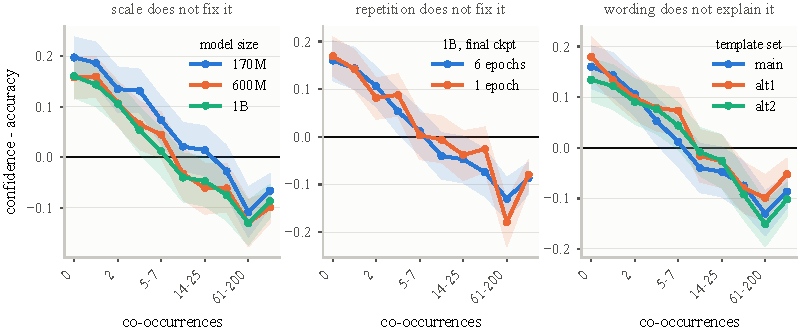
\includegraphics[width=\textwidth]{figures/fig5_controls.pdf}
\caption{The gap under three controls. Model size, number of epochs and prompt wording all leave
the pattern intact.}
\label{fig:controls}
\end{figure*}

\subsection{Where the wrong answers come from}
\label{sec:prior}

If confidence arrives before knowledge, something must be supplying the answers. We test whether
wrong choices fall on the option the model would favour with no subject at all, scoring each
candidate under the neutral prompt \textit{The answer is} and taking the highest-scoring
distractor as the model's prior for that relation.

Among wrong answers, 52.0\% land on that option, against 11.1\% expected by chance
($p < 10^{-300}$, binomial). The rate peaks at 0.566 in the middle of the range and falls to
0.357 in the most frequent bin (Figure~\ref{fig:prior}). Using corpus frequency to define the prior instead
of the model's own preference gives the same trend at a lower rate. Errors on rare entities are
therefore closer to a default guess for the relation, while errors on well-attested entities look
more like specific confusions.

\begin{figure}[t]
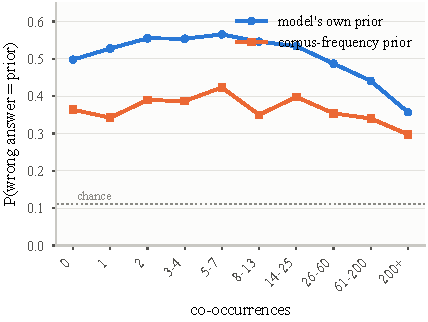
\includegraphics[width=\columnwidth]{figures/fig6_prior_collapse.pdf}
\caption{Share of wrong answers that match the model's preferred answer for the relation,
measured with no subject in the prompt. Chance is 0.111.}
\label{fig:prior}
\end{figure}

\subsection{Predicting errors}
\label{sec:pred}

We ask whether the quantities above predict failures on held-out entities. The label comes from
free generation, namely whether the model produces a wrong answer, while the features come from
the multiple-choice probe and from corpus counts, so no predictor has access to its own label.


Results are in Table~\ref{tab:baselines}. Co-occurrence count alone reaches 0.784 ROC-AUC and
probe confidence alone reaches 0.868, both well above the majority-class baseline. Combining them
changes little, and the difference of 0.016 has a bootstrap interval spanning zero. Because
86\% of test facts are errors, accuracy and F1 are close to uninformative here.

\begin{table}[t]
\centering\small
\begin{tabular}{lrl}
\toprule
\textbf{Predictor} & \textbf{AUC} & \textbf{95\% CI} \\
\midrule
Majority class  & 0.500 & \\
Co-occurrence   & 0.784 & [0.721, 0.842] \\
Probe confidence& \textbf{0.868} & [0.829, 0.906] \\
Both            & 0.852 & [0.799, 0.899] \\
\bottomrule
\end{tabular}
\caption{Predicting free-generation errors on held-out entities, final checkpoint. ``Both'' is a
logistic regression on the two features. The positive rate is 86.4\%, so accuracy and F1 are
uninformative here and are omitted. Intervals are bootstrapped over the 757 test facts.}
\label{tab:baselines}
\end{table}

The picture changes if we ask about confident errors rather than errors. Restricting to
generations the model is sure about, the rate does not fall with frequency but peaks in the
middle, at 0.360 for facts with 61--200 co-occurrences against 0.238 for facts with none, measured
over all 2{,}993 facts rather than the held-out split.
Bootstrap intervals over facts are 0.307 to 0.413 and 0.191 to 0.289, and the difference of 0.122
has an interval of 0.048 to 0.195. The ordering holds at the 50th, 75th and 90th percentiles of
generation confidence. Producing a confidently wrong answer seems to need enough
familiarity to construct a specific one. For the rarest entities the model tends to generate
vague text instead.

\section{Discussion}

An untrained model is already overconfident, and uniformly so. What training supplies, and only
where the corpus supports it, is the accuracy that would justify that confidence. Where it
arrives the two align. Where it does not, the initial overconfidence simply stays.

The gap on rare entities is therefore a property of the training data rather than of a
particular model. Nothing we varied removed it: a six-fold increase in parameters moved the
rare-end gap by 0.037, and six passes over the corpus moved it less. \citet{kandpal-etal-2023-large} estimate that reaching high accuracy on long-tail questions
would need models many orders of magnitude larger than current ones. Over the range we tested,
scale does little for long-tail calibration.

One result runs against the pattern and we do not have a confident explanation. The gap in the
most frequent bin ($-0.087$) is smaller in magnitude than in the 61--200 bin ($-0.130$), so
underconfidence peaks just below the top of the range rather than at it. This reversal appears in
all four models we tested, so it is unlikely to be noise. A plausible reading is that at the highest
frequencies the model is accurate enough that confidence starts catching up again, but we did not
test this.

The two probing methods disagree. In multiple choice, where the model
must distribute mass over a fixed set, overconfidence is largest for the rarest facts. In free
generation, confident errors are most common in the middle of the frequency range. Both can be
true: the multiple-choice setting forces a commitment that free generation does not, and a model
with no information about an entity produces hedged text rather than a confident falsehood. Which
setting is the better model of deployed behaviour depends on the application.

\section{Conclusion}

Confidence and accuracy come apart during pretraining, and how far they come apart is predictable
from a count that can be computed before training finishes. The separation is established within
the first 1{,}000 of 658{,}032 steps, and survives changes in model size, epoch count and prompt
wording. When the model does err on a rare entity, it falls back on its default answer for the
relation more often than on anything specific to the entity asked about.

\section*{Limitations}

Our models are small by current standards, at most 1B parameters, and are trained on Wikipedia
alone. Whether the same pattern holds for models trained on mixed web corpora is untested.
\citet{gottesman-etal-2026-lment} do report the same frequency-performance trend for models
trained on broader data, but they score those models against their own Wikipedia-derived counts
rather than counting the other corpora. What happens when the corpus itself changes is still
open.

We can locate the onset of confidence no earlier than step 1{,}000, because that is the finest
public checkpoint spacing, and it is available for only one of the four models. Most of the rise
happens before that point, so we can say the separation is established early but not how early.

The ten-way multiple-choice probe is a convenient measurement, not a realistic task. It supplies
a fixed candidate set that a deployed model would not have, and our free-generation results show
the two settings do not always agree.

The lowest frequency bin is not a zero-knowledge control. Its accuracy is 0.181 against a chance
level of 0.100, since the subject entity usually appears in the corpus even when it never
co-occurs with the answer. That is not the whole story: on the 112 facts whose subject is absent
entirely, accuracy is 0.205 [0.134, 0.286], which overlaps the bin rather than falling below it.
The gap there is $+0.124$, so the pattern holds, but we cannot attribute the above-chance
accuracy to subject exposure.

Co-occurrence count is correlated with how often the answer string appears on its own, so part
of the trend we report may reflect familiarity with the answer rather than knowledge of the
fact. Section~\ref{sec:prior} is consistent with that concern but does not settle it, and we
did not run a probe that separates the two.

Finally, we cover 16 relations from one English dataset, and the probe set was generated from a
single random seed. We report results for one seed rather than an average over several.

\section*{AI Disclosure and Reflection}

We used Claude Code (Opus 5) as a helper throughout the project: for writing and debugging the
notebook code, including the parts using HuggingFace and PyTorch libraries we had not worked with
before, for producing the figures, for drafting and tidying the prose, and for discussing how to
read the results.

The main lesson was that its output needs checking rather than trusting. It was reliable on code
and library details, and least reliable with numbers. Several values were attributed to the wrong
frequency bin, and quantities quoted in the text did not always match the tables they came from.
We caught these by recomputing everything from the saved per-fact results and reading the tables
against the text.

\section*{Acknowledgments}

We thank the authors of LMEnt for releasing the models, corpus annotations and checkpoint
metadata that this project depends on.

\bibliography{custom}

\end{document}
